\documentclass{wileySix}
\usepackage{w-bookps}

% \usepackage{mathptmx}

\usepackage{graphicx}
\usepackage{enumitem}

\setcounter{secnumdepth}{3}

\setcounter{tocdepth}{2}

\begin{document}

\booktitle{Web Service}
\subtitle{Semua Tentang Komunikasi antar Aplikasi Berbasis Protokol internet}

\author{Rolly Maulana Awangga}

\halftitlepage
\titlepage



\offprintinfo{Web Service, pre-release}{Rolly Maulana Awangga}


\begin{copyrightpage}{2018}
Web Service / Rolly Maulana Awangga
\end{copyrightpage}


\dedication{For my family}

\contentsinbrief %optional
\tableofcontents
\listoffigures %optional
\listoftables  %optional

%%%%%%%%%
%%Content 
%%%%%%%%%

\part[Pengenalan Web Service]
{Pengenalan\\ Web Service}

%\chapter[Contoh]
%{Contoh\\ Latex}
%tugas 1 :
Tuliskan resume atau tutorial;

2A :
1. Python instalasi dan definisi dan contoh kode awal
2. wsgi definisi dan contoh contoh
3. cgi definisi dan contoh
4. uwsgi instalasi definisi dan contoh
5. Install the Windows Subsystem for Linux


2B :
1. contoh aplikasi web service
2. pengertian web service
3. protokol
4. port
5. penggunaan aplikasi testing web service


2C :
1. internet
2. web
3. backend
4. frontend

Syarat :
1. gunakan SPOK yang benar
2. Tanda baca yang benar
3. Penggunaan Huruf kapital yang benar

buat grup kelompok di github dan fork webservice

Parameter(baca standar penulisan latex) :
1. itemize dan enumerate yang benar (10)
2. gambar dan referensi disebutkan dalam kalimat dengan benar (10)
3. penggunaan section subsection subsubsection yang benar (10)
4. Penggunaan tabel atau verbatim atau equation (10)
5. commit sehari(min 50 kata) per anggota kelompok selama 6 hari (60)

Nilai akhir X persentasi plagiarisme = Nilai tugas

(GUnakan standar penggunaan git)
jika ada error maka minus 5 setiap kali pull request

%\chapter[Internet]
%{Definisi\\ Internet}
%%\begin{itemize}
%\item Ahmad Syafrizal Huda (1164062) 
%\item Annisa Fathoroni (1164067) 
%\item Puad Hamdani (1164084) 
%\item Rahmi Roza (1164085) 
%\item Tasya Wiendhyra (1164086) 
%\end{itemize}

Pada gambar \ref{labelgambar} merupakan gambar inspirasi tentang internet.
\begin{figure}[ht]
\centerline{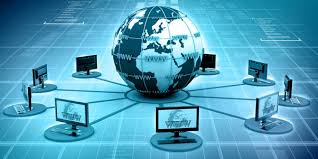
\includegraphics[width=1\textwidth]{figures/1internet.JPG}}
\caption{Internet}
\label{labelgambar}
\end{figure}

\section{Pengertian Internet}
\paragraph{} Secara harfiah internet adalah kependekan dari interconnected network yang berarti rangkaian komputer yang terhubung satu sama lain. Hubungan melalui suatu sistem antar perangkat komputer untuk lalu lintas data itulah yang dinamakan network. Sebagai contoh yaitu LAN, MAN dan WAN. Misalnya LAN. LAN merupakan singkatan dari Local Area Network yang menghubungkan komputer atau jaringan dalam area tertentu seperti kantor, sekolah atau warnet. Jadi komputer yang terhubung melalui satu jaringan dan saling berkomunikasi dengan waktu dan wilayah yang tidak terbatas, disebut internet.
Internet, sebagai teknologi yang melalui proses pengalihan dari tempat lahirnya ke Indonesia, mengalami proses transformasi dan lokalisasi yang terjadi dalam arena perebutan kekuasaan politik antara negara, korporasi, dan masyarakat sipil. Di dalam arena perebutan kekuasaan ini, titik utama pergulatan ini adalah pembentukan dan penegasan identitas. Berdasarkan pengalaman historis yang ada di Indonesia, tulisan ini mengungkapkan bagaimana internet bersisian dengan pergulatan identitas dan pembentukan komunitas politik yang mandiri di luar negara dan korporasi.
\cite{darma2009buku}.

\section{Sejarah Internet}
\paragraph{} Sejarah Internet : Rangkaian pusat yang membentuk internet diawali pada tahun 1969 oleh ARPA (Advance Research Project Agency), sebuah badan yang dibentuk pada tahun 1958 oleh Amerika yang terdiri dari para peneliti dan teknisi dari universitas dan laboratorium yang ada di Amerika. Awalnya badan ini dibentuk untuk menyaingi Rusia, yang saat itu lebih maju dibidang satelit. Para peneliti bekerja, tidak harus di satu lokasi, untuk membuat penelitian dan mendedikasikan hasil penelitian tersebut untuk perkembangan teknologi Amerika Serikat.

\section{Manfaat Internet}
\paragraph{} Internet di dunia bisnis untuk pergantian informasi, pencatatan produk,media yang mempromosikani, surat elektronik, bulletin boards, kuesioner elektronik, dan mailing list. Biasanya digunakan untuk berkomunikasi,berdiskusi, dan dilibatkan secara proaktif dan interaktif dalam perancangan, pengembangan,pemasaran, dan penjualan produk. Pemasaran melalui internet terdapat 2 metode, yaitu push dan pull marketing. keutamaan dari perencanaan bisnis yang didapat di internet ialah komunikasi dunia dan interaktif diantaranya, serta menyediakan informasi penting dan pelayanan yang sesuai dengan kebutuhan konsumen, juga meningkatkan kerja sama.
\cite{yuliana2004penggunaan}.

Pada table \ref{table:contoh} merupakan Klasifikasi Dimensi Kepentingan Penggunaan Internet.
\begin{table}[h]
\centering
\begin{tabular}{|c|c|}
\hline
Dimensi Kepentingan Penggunaan Internet&Contoh Aktivitas Internet\\
\hline
Informasi&Memperoleh informasi atau berita online\\
Kesenangan&Online untuk alasan yang tidak istimewa,hanya untuk kesenangan atau untuk mnghabiskan waktu\\
komunikasi&Mengirim atau menerima pesan,misalnya email\\
Transaksi&Membeli produk secara online, misalnya buku, musik, mainan atau pakaian\\
\hline
\end{tabular}
\label{table:contoh}
\end{table}

\section{Macam-macam Internet}
\subsection{IOT}
\paragraph{} Internet of Things (IOT) merupakan perkembangan keilmuan yang sangat menjanjikan untuk mengoptimalkan kehidupan berdasarkan sensor cerdas dan peralatan pintar yang bekerjasama melalui jaringan internet (Keoh, Kumar, dan Tschofenig, 2014).Menurut (Burange dan Misalkar, 2015) Internet of Things (IOT) adalah struktur di mana objek. orang disediakan dengan identitas eksklusif dan kemampuan untuk pindah data melalui jaringan tanpa memerlukan 2 arah antara manusia ke manusia yaitu sumber ke tujuan atau interaksi manusia ke komputer.
\cite{junaidi2015internet}.
\subsection{ISP}
\paragraph{} Internet Service Provider (ISPs) menghubungkan pengguna dengan perusahaan/pebisnis provider ke internet yang luas atau lebih dikenal dengan internet publik. Para perusahaan ini harus bersaing satu sama lainnya dalam harga, kecepatan, kinerja, dan lainnya. Tetapi mereka pun harus bekerja sama dalam menyediakan konektivitas global dengan semua hal yang berkaitan dengan internet. Tier 1 ISP adalah ISP yang memiliki hak untuk mengakses ke dalam routing internet global tapi tidak membeli transit atau pemberhentian apapun dari orang lain atau pihak lainnya.
\cite{norton2001internet}.
\subsection{Internet Banking}
\paragraph{} Internet Banking ataupun Online Banking didefinisikan sebagai portal dalam internet yang digunakan kostumer untuk melakukan pembayaran, transaksi, untuk berinvestasi. Perkembangan Internet Banking ini dalam hal keuangan dan per bankan membuat cara baru untuk melakukan dan mengatasi permasalahan yang ada pada sehari hari. Penerimaan Internet Banking dalam kalangan masyarakat disambut baik, dan peluasan kontrak e-banking di seluruh dunia saat ini sudah mencapai 50 persen.
\cite{pikkarainen2004consumer}.
\subsection{Cybercrime}
 Cybercrime merupakan kejahatan yang beberapa tahun belakang ini terjadi, media yang digunakan yaitu internet. Kejahatan yang dilakukan beragam, mulai dari mencuri atau mengambil uang dari rekening seseorang, melakukan Bullying, kejahatan seperti menerbitkan video atau pun gambar asusila yang melanggar norma -  norma yang berlaku, sampai menyelundup kedalam properti ataupun jaringan seseorang dan mengakibatkan kerusakan seperti memasukan virus, dan hacking.
\cite{yar2005novelty}.

\section{Pengaruh dan Dampak Internet}
\paragraph{} Pengaruh dan dampak internet sebagai alat media komunikasi. Seperti halnya media massa yang lain, keberadaan internet ini membangkitkan berbagai pertanyaan akan efek negatif yang ditimbulkannya, selain keberadaan efek positif seperti penyampaian dan pengiriman informasi yang cepat dan update melalui fasilitas-fasilitas e-mail, sural kabar online, forum diskusi dan juga chatting serta beragam situs-situs yang ada yang memperkaya khasanah pengetahuan penggunanya. Lebih lanjut keberadaan media komunikasi ini seringkali dianggap sebagai penyebab perilaku asosial penggunanya.
Dampak internet, pemasaran terhadap perusahaan, produk, dan pelayanan menjadi proses yang interaktif saat ini. Situs Web perusahaan bukan hanya sekedar menyajikan katalog produk dan media promosi, melainkan digunakan untuk berdialog, berdiskusi, dan berkonsultasi dengan konsumen secara On-line, bulletin boards, kuesioner elektronik, mailing lists, dan pengiriman surat elektronik. Sehingga semua konsumen dapat dilibatkan secara langsung dalam perancangan, pengembangan, pemasaran, dan penjualan produk.
\cite{surya2009pola}.

\section{Koneksi Ke Internet}
\paragraph{} Ada beberapa macam koneksi yang dapat dilakukan agar anda dapat terkoneksi dengan internet, dan melakukan aktivitas online sepuasnya. Jenis-jenis koneksi juga menentukan kecepatan akses internet anda, dan tentu saja membutuhkan biaya. Perlu diperhatikan pada kecepatan akses, KBps kependekan dari kilobit per second (kilobit per second), yang berbeda dari KBps (kilobyte per second/kilobita per detik), dimana 1 bita sama dengan 8 bit.

\section{Cara Menyimpan Data Ke Internet}
\paragraph{} Ketika mengerjakan file di komputer, membuat sistem back-up, sehingga jika file asli mengalami kerusakan, masih mempunyai file cadangan dan data-data tidak hilang seluruhnya. Memang, bukan berarti membuat Salinan sudah pasti aman, tetap saja ada resikonya, bila semua file di komputer dan flashdisk juga terkena virus. Oleh karena itu, harus memiliki sistem back-up lain. Salah satu cara yang bias dilakukan adalah menyimpannya data di dalam internet.
\cite{lim2014informational}.

\section{Keamanan Internet}
\paragraph{} Untuk melihat keamanan sistem internet perlu diketahui cara kerja internet. Antara lain yang perlu diperhatikan adalah hubungan antara komputer di internet, dan protokol yang digunakan oleh semua orang (public). Untuk mencapai server tujuan, paket informasi harus melalui beberapa sistem yang kemungkinan besar berada di luar kontrol dari kita. Setiap titik yang dilalui memiliki potensi untuk dibobol, disadap, dipalsukan.
\cite{rahardjo2002keamanan}.

\section{Perbedaan Internet dan Media Komunikasi Klasik}
Perbedaan Internet dari media komunikasi klasik dalam penggunaanya:
\begin{itemize}
\item Pengguna internet sebagai perantara untuk berkomunikasi menuntut penggunannya memiliki pengetahuan bagaimana cara menggunakan software baik itu komputer maupun smartphone mereka secara umum dan software aplikasi internet secara khusus.
\item Komunikasi dalam internet selain memiliki konteks komunikasi massa, juga membentuk komunikasi personal dalam jumlah banyak
\item Sifat dan bentuk pesan-pesan yang disampaikan melalui semua media komunikasi dimiliki oleh medium internet
\item Dalam komunikasi melalui internet memungkinkan terjadinya komunikasi antar berbagai personal atau hubungan lain yang memiliki perbedaan, baik itu secara sosiologis maupun budaya.
\end{itemize}
\cite{effendi2009peranan}.

\section{Kelebihan dan Kekurangan Internet}
\subsection{Kelebihan Pada Internet}
    Kelebihan internet sebagai media baru dalam pembelajaran dapat kita lihat sebagai berikut:
\begin{enumerate}
\item Kita bisa menyebarluaskan informasi yang bisa di akses dari mana saja di seluruh dunia dalam waktu singkat.
\item Kita bisa berkomunikasi secara langsung melalui telepon dan unit video processing. Kita bisa melakukan chat melalui jaringan gratis chat yang sangat luas yaitu mIRC.
\end{enumerate}
\subsection{Kekurangan Pada Internet}
    Selanjutnya dapat pula kita lihat kekurangan internet sebagai media baru dalam pembelajaran  sebagai berikut:
\begin{enumerate}
\item Sebagai ajang debat kusir yang berkepanjangan. Ironisnya, debat ini sering kali bersembunyi atas hak anonimitas.
\item Fitnah di era digitalisasi memang menjadi sesuatu yang murah dan diumbar oleh siapa saja tanpa pembuktian yang jelas.
\end{enumerate}
\cite{gafar2017penggunaan}.



%\chapter[Web]
%{Definisi\\ Web}
%%\begin{itemize}
%\item Imron Sumadireja (1164076)
%\item Jesron Marudut (1164077)
%\item Lusia Violita Aprilian (1164080)
%\item Mhd. Zulfikar Akram Nst. (1164081)
%\end{itemize}

\section{Pengertian Website}
World wide web (www atau web) merupakan halaman situs informasi yang dapat diakses secara cepat atau sarana
antar muka informasi di internet. Web dapat menggabungkan teks, grafik, dan multimedia. Web memudahkan
penggunanya untuk mengakses informasi melalui konsep hypertext sehingga memungkinkan  suatu text untuk
menjadi acuan membuka dokumen laindo. Informasi dapat mudah disebar dan diakses.

\subsection{Sejarah Website}
Sementara itu World wide web (www) dikembangkan pertama kali oleh Tim Berners-Lee pada tahun 1989. Pada
awalnya, Tim mengusulkan WWW sebagai suatu cara berbagai dokumen diantara para peneliti. Dokumen online dapat
diakses melalui alamat unik yang disebut Universal Resource Locator atau URL. Selain itu WWW tidak hanya
dikembangkan untuk keperluan para peneliti, namun juga dikembangkan untuk kalangan pendidikan, bisnis dan
perorangan. Berdasarkan penjelasan singkat diatas dapat disimpulkan bahwa antara web dan internet memiliki
hubungan yang sangat erat walaupun keduangnay tidak bisa dikatakan sama. Web merupakan bagian dari layanan
yang dapat berjala di atas teknologi internet.

\subsection{Jenis-jenis website}
Website dikelompokan dalam beberapa jenis-jenis Website agar dapat memudahkan dalam menentukan jenis website
yang akan ditentukan. Dan berikut jenis-jenis website yang dikelompokan atas beberapa dasar:
\begin{enumerate}
\item Jenis Website berdasarkan sifat;
\begin{itemize}
\item Website Statis, merupakan web yang kontenya hampir jarang diubah
\item Website Dinamis, Web yang konten atau isinya dapat berubah-ubah setiap saat
\end{itemize}
\item Jenis Website yang dikelompokkan berdasarkan Bahasa Pemrogramannya;
\begin{itemize}
\item Server side, Website yang memakai bahasa pemrograman yang tergantung dengan servernya
\item Client side, adalah web yang tidak perluu server untuk menjalankannya. Cukup diakses dengan browser.
\end{itemize}
\item Jenis-jenis Web menurut tujuannya;
\begin{itemize}
\item Web personal, biasanya web ini merupakan web yang berisi informasi seorang
\item Corporate Web, website yang dimiliki sebuah institusi atau perusahaan.
\item Web Portal, Web ini berisi banyak layanan, seperti berita, email dan jasa
\item Web Forum, sebuah web yang dibuat sebagai sarana diskusi.
\end{itemize}
\end{enumerate}
	
\subsection{Keuntungan Web}
Keuntungan penggunaan web diantaranya yaitu :
\begin{itemize}
\item Informasi dapat diberikan segera(tepat waktu) dan diperbarui secara berkala.
\item Presentasi fleksible dan visibilitas dapat menyediakan ragam isyarat untuk diseminasi informasi.
\item Informasi dapat diorganisir melalui tautan dan menu, berbagai tingkatan informasi dapat disediakan format file yang berbeda dapat digunakan untukj informasi yang dapat diunduh. Integrasi informasi dapat dilakukann melalui tautan dan seksi lain, halaman lain, atau web lain.
\item Tauta  dan menu dapat menyediakan informasi bagi pemangku kepentingan yang berbeda, informasi dapat pula diberikan melalui daftar email kepada pemangku kepentingan.
\item Setiap orang yang dapat mengakses web dapat memperoleh informasi karena keterjangkauan global dan potensi komunikasi masl dari web.
\end{itemize}
	   
\section{tentang web scraping}
Web scraping atau scraping web (dapat disebut juga panen web atau web ekstraksi data) merupakan sebuah
perangkat lunak komputer teknik penggalian informasi dari situs web seperti mengambil mengambil data
berbentuk teks yang umumnya bertipe HTML atau XHTML. contohnya seperti Internet Explorer (IE) dan Mozilla Web
Browser. web scraping berkaitan erat dengan pengindekan web.

\subsection{manfaat dari web scraping}
Web scraping sering dikenal dengan screen scraping. Web scraping tidak dapat dimasukkan kedalam bidang data
mining karena dalam data mining menyiratkan upaya untuk memahami pola semantik dari sejumlah data besar yang
telah diperoleh. Aplikasi Web scraping hanya fokus pada cara memperoleh data melalui pengambilan dan ekstrasi
dengan ukuran data yang bervariasi. Manfaat dari web scraping adalah agar informasi yang diambil lebih
terfokus sehingga dapat memudahkan dalam melakukan pencarian sesuatu, adapun cara untuk mengembangkan teknik
web scraping yaitu dengan cara sebagai berikut:
\begin{enumerate}
\item Pengembang/pembuat program mempelajari dokumen HTML dari website yang akan diambil informasinya untuk
di tag HTML tujuannya yakni untuk mengapit informasi yang akan diambil (Create Scraping Template)
\item Pengembang/pembuat program mempelajari teknik navigasi pada website yang akan diambil informasinya
untuk ditiru pada aplikasi web scraping yang akan dibuat (Explore Site Navigation)
\item Selanjutnya aplikasi web scraping akan mengotomisasi informasi yang didapatkan dari website yang telah
ditentukan (Automate Navigation and Extraction), informasi yang didapat tersebut akan disimpan dalam 
tabel basis data (Extracted Data and Package History).
\end{enumerate}

\subsection{Perbandingan Metode Web Scraping}
Berikut perbandingan antara metode Web Scraping menggunakan CSS Selector dan Xpath Selector
\begin{enumerate}
\item Penggunaan metode XPATH Selector untuk web scraping menghasilkan artikel yang lebih lengkap
dibandingkan dengan menggunakan metode CSS Selector, Ditunjukkan dengan jumlah item dan ukuran file
yang didapatkan lebih besar. Namun juga menyisakan proses lain untuk menghilangkan kode HTML yang tidak
diinginkan dari artikel yang dihasilkan menggunakan metode XPATH Selector.
\item Dalam penggunaan memori baik metode XPATH Selector dan CSS Selector tidak memiliki perbedaan yang
signifikan(cenderung sama). Disebabkan karena engine scrapy yang baik dalam penggunaan resource-nya. 
\item Metode XPATH Selector memiliki waktu proses yang lebih cepat daripada menggunakan metode CSS Selector.
\item Pada metode XPATH, selector cukup mengikuti node pada halaman web, sehingga waktu yang dibutuhkan
relatif lebih singkat.
\end{enumerate}

\section{Tentang Web Hosting}
Web hosting merupakan jasa penyewaaan tempat penyimpanan data di internet atau biasa disebut dengan cloud
yang diperlukan oleh sebuah website. Web hosting ialah salah satu syarat agar website bisa diakses secara 
online dan dapat diakses dari seluruh dunia. Ukuran yang digunakan dalam suatu web hosting adalah kapasitas
dan bandwidth. Kapasistas merupakan ukuran besarnya kemampuan sebuah web hosting untuk menyimpan data-data di internet.

Bandwidth merupakan ukuran maksimal dari jumlah volume data yang diperbolehkan untuk diakses dari web hosting
setiap bulannya. Sebagai contoh, sebuah halaman website yang mempunyai ukuran 2 MB dan bandwidth web hosting
2000 MB, maka setiap bulannya website tersebut dapat diakses sebanyak 2000 kali.

\subsection{Tentang Domain}
Domain merupakan sebuah alamat di dunia internet atau sebuah identitas dari sebuah website. Domain digunakan untuk mempermudah dalam mengakses situs yang ada di internet. Domain terbagi menjadi 2 jenis domain yang dibagi berdasarkan pemisahaan titiknya, yaitu; Top Level Domain (TLD) dan Second Level Domain (SLD). Top Level Domain merupakan bagian terakhir dalam sebuah domain website. Contohnya "facebook.com" dan disitu yang jadi domainnya adalah ".com". Selanjutnya Second Level Domain atau SLD merupakan bagian dari domain yang terdapat sebelum Top Level Domain. Contohnya "Facebook.com" yang menjadi SLDnya adalah Facebook. Jadi SLD adalah unsur domain yang didaftarkan terdahulu pada jasa Web Hosting. Dan ada juga yang disebut Country Code Second Level Domain (ccSLD). Berguna sebagai penunjuk organisasi apa yang mendaftar pada suatu domain. Setiap negara juga mempunyai ccSLD yang berbeda-beda tiap negaranya.

\subsection{Tentang Hubungan Domain dan Web Hosting}
Hubungan Domain dan Web Hosting merupakan satu kesatuan yang saling membutuhkan. Pada sebuah Website, domain dan web hosting saling ketergantungan. Apabila yang tersedia hanya web hosting, maka website tidak akan dapat diakses. Begitu juga dengan domain, apabila yang tersedia hanya domain, maka tidak akan ada website yang akan ditampilkan, karena halaman website tersimpan didalam web hosting.

\subsection{Macam-macam Web Hosting}
Saat ini banyak jasa penyedia hosting dengan harga relatif murah bahkan gratis. Berikut adalah macam-macam web hosting :
\begin{enumerate}
\item Free Hosting / Web Hosting Gratis
Dengan free hosting, kita dengan mudah mencari layanan web hosting dan domain gratis di internet dengan menggunakan fasilitas search engine seperti google atau yang lainnya. Biasanya penyedia web hosting tidak mengenakan biaya. Namun, memiliki banyak keterbatasan beberapa fitur.
\item Web Hosting Berbagi atau Shared Hosting
Jenis hosting ini paling sering digunakan karena bukan hanya murah, namun juga memiliki layanan yang  dapat mencukupi segala kebutuhan. Biasanya, untuk menggunakan layanan web hosting ini anda hanya perlu untuk mengeluarkan biaya sebesar 100 hingga 200 ribu untuk mendapatkan ruang sebesar 2 GB – 7,5 GB dengan bandwith unlimited.
\item VPS Web Hosting
VPS merupakan singkatan dari Virtual Private Server. Jadi disini anda dapat seperti memiliki server sendiri untuk situs anda. dengan server ini, anda akan memiliki control yang lebih dalam seperti Dedicated Server.
\item Dedicated Web Hosting
Dedicated Web Hosting merupakan sebuah layanan hosting dengan server yang memiliki kemampuan untuk melakukan handle terhadap traffic dengan jumlah sangat banyak. Serta memiliki banyak fitur premium di dalamnya. Selain itu,juga memiliki control penuh terhadap server walaupun  hanya menyewanya.
\item Managed Web Hosting
Managed Hosting / Web Hosting Terkelola ini adalah web hosting yang dikhususkan untuk situs dengan. Platform yang sama. Managed web hosting biasanya lebih aman dan kinerjanya lebih optimal. Selain itu, memudahkan untuk melakukan beragam pengaturan, mulai dari installasi, sampai setting macam-macamnya.
  \end{enumerate}

\subsection{Cara Mendapatkan Web Hosting dan Domain}
Web hosting dan domain lebih sering ditemukan oleh perusahaan-perusahaan penyedia web hosting atau domain. Untuk menemukannya, cukup cari di google. Maka akan banyak perusahaan yang menyediakan jasa web hosting. Kinerja web hosting berbeda-beda dari setiap perusahaan Web hosting. Karna apabila web hosting yang dibuat oleh jasa tersebut buruk maka website tersebut akan mudah bermasalah. Oleh karena itu dalam pembelian jasa domain atau web hosting perlu diperhatikan hal-hal seperti profil dari penjual web hosting, fitur untuk website dan harga dari web hosting tersebut. Dalam memilih penyedia web hosting, pastikan penyedia mempunyai reputasi yang bagus dan terpercaya. Dan sebaiknya memilih perusahaan web hosting yang sudah dalam bentuk perusahaan CV atau PT agar pertanggung jawabannya jelas ketika terjadi gangguan web hosting.
	
\section{Apa itu cPanel?}
Apa itu cPanel?
cPanel adalah perangkat lunak control panel online untuk melakukan pengaturan website dalam sebuah web histing. cPanel adalah tool utama untuk pengguna web hosting. 
Beberapa fungsi utama cPanel antara lain yaitu upload data website, pengaturan data website, instalasi content management system, dan lain-lain. Melelui cPanel juga kita bisa mengatur data-data website. Kita bisa menambah, menghapus, atau memodifikasi data website.

\subsection{Backup date dengan cPanel}
Kemudahan yang diberikan cPanel sebagai control panel yakni untuk mempermudah proses hosting di suatu situs web menggunakan 3 tingkatan struktur untuk memberikan fungsi administrator, agen, dan yang memiliki situs web tersebut untuk mengatur berbagai macam aspek dari situs web dan administrasi server melalui sebuah web standar. Dalam menu cPanel untuk backup disediakan 3 pilihan layanan backup yang ada yakni:
\begin{enumerate}
\item System Backup, merupakan menu backup yang dapat digunakan untuk mendownload backup otomatis yang telah dibuat oleh administrator server
\item Full Backup, akan melakukan backup file untuk mengembalikan file yang corrupt, terhapus atau pindah pada server yang lain.
\item Backup Home Directory, berfungsi untuk memberikan hak akses untuk mengambil file yang berada pada directory home.
\end{enumerate}


\chapter[Backend]
{Definisi\\ Backend}


\section{Backend}

\begin{figure}[ht]
\centerline{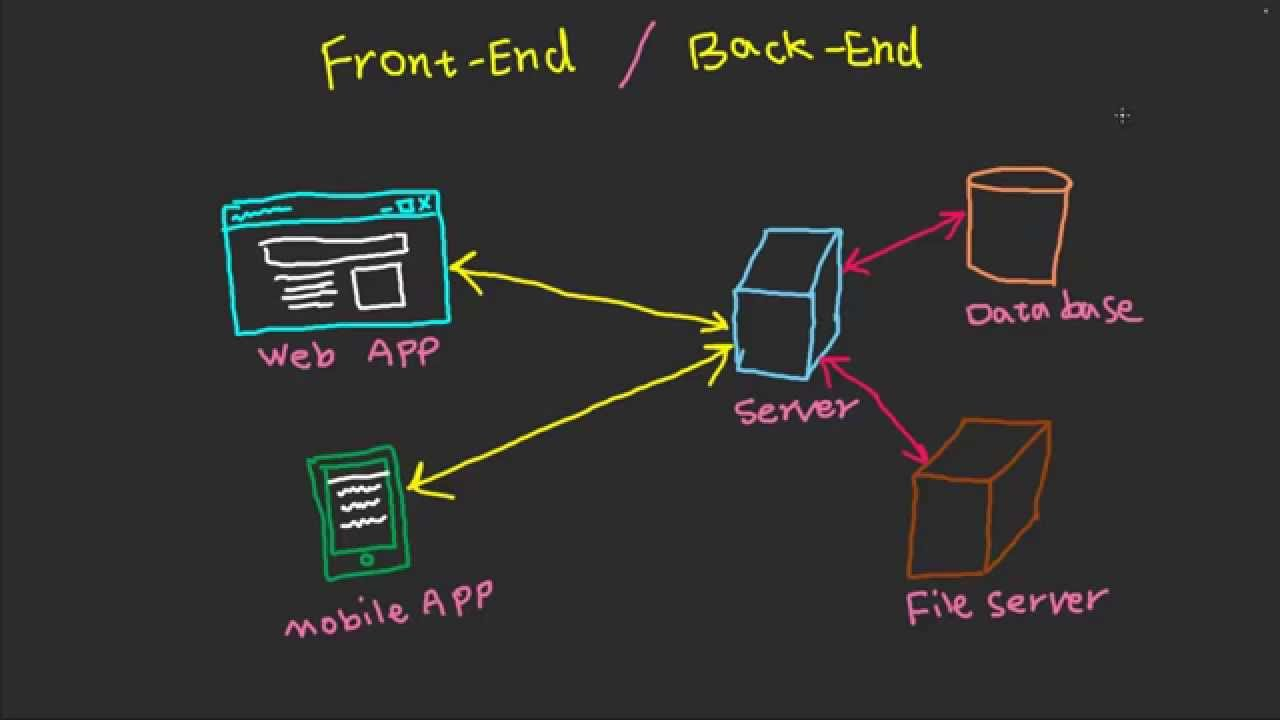
\includegraphics[width=1\textwidth]{figures/1backend.jpg}}
\caption{Backend}
\label{1backend}
\end{figure}

	Pada gambar \ref{1backend} berikut ini dijelaskan mengenai Back-end atau server-side yang merupakan bagaimana sebuah website berkerja, meng-update
dan berubah. back-end adalah sesuatu system yang dimana User tidak akan dapat melihatnya di dalam browser,
seperti Database dan Server. biasanya orang - orang yang bekerja di bagian back-end di panggil atau disebut sebagai
Programmers atau Developer. Back-end developers adalah orang yang paling khawatir tentang hal - hal yang menyangkut keamanan,
struktur sistem dan manajemen konten. sebenarnya para back-end develper juga mengetahui tentang front-end seperti HTML dan CSS.
namun itu bukanlah bidang mereka bekerja. 

\subsection{Backend System}
	Pada system dan metode  yang membuat informasi dapat digunakan secara oromatis untuk mengakses 
pada fungsionalitas system computer backend yang digunakan ke server aplikasi. 
Metode ini juga dapat beroperasi untuk menghubungkan ke system computer backend dan memperoleh 
fungsionalitas untuk menentukan informasi  pada system backend. Dan pada informasi yang diperoleh 
dan dapat dianalisis secara terprogram,dan informasi yang sangat baru dapat dianalisis yang dimana 
informasi dibuat secara terprogram dapat digunakan untuk mengakses fungsionalitas system backend.
Back-end biasanya mengacu pada program dan skrip yang bekerja di dalam server, untuk membuat sebuah 
halaman web yang dinamis dan interatif. Back-end memiliki tugas-tugas yaitu seperti :

\begin{enumerate}
\item Desain Informasi pada web
\item Pemrosesan form
\item Pemrograman dalam database
\item Aplikasi Berbasis Web
\end{enumerate}
Dari tugas - tugas tersebut Back-end memiliki tiga bagian diantaranya yaitu server,aplikasi, dan database
\cite{shapiro2005system}.

\section{Bahasa Pemrograman yang digunakan di Backend}
Pada gambar \ref{2labelgambar} berikut ini dijelaskan bahwa pada Backend terdapat beberapa bahasa programing yang digunakan,
termasuk C, Python, dan lainnya. pada materi di bawah ini terdapat beberapa penjelasan tentang bahasa pemrogramannya.

\begin{figure}[ht]
\centerline{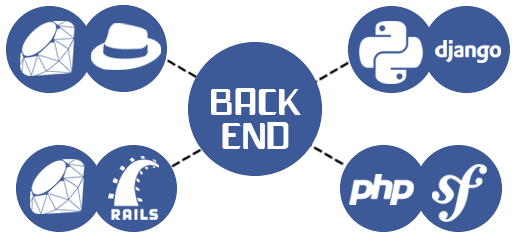
\includegraphics[width=1\textwidth]{figures/1bahasapemrogramanbackend.png}}
\caption{Bahasa Pemrograman yang dipakai di Backend}
\label{2labelgambar}
\end{figure}

\subsection{C}
	Bahasa Pemrograman Backend yang biasa digunakan developer ialah C, C++, dan Java .
Bahasa C adalah suatu perkembangan dari bahasa B yang di kembangkan oleh Ken Thompson pada tahun 1980.
Bahasa C rilis pertama kali ditulis oleh Brian W. Bahasa C, awalnya digunakan oleh sistem operasi UNIX.
Bahasa C adalah bahasa pemrograman tingkat standar, bahasa C memiliki kegunaan yang sering di gunakan
diantaranya untuk membuat perangkat lunak.

\subsection {C++}
	Pengertian C++ adalah `multi-paradigm' artinya anda dapat menulis suatu kode, caranya procedural 
tapi juga bisa menggunakan fungsional,berorientasi objek, dan campuran paradigm suatu pemrograman.  
Bahasa pemrograman C++ ini bisa lebih sulit untuk dipelajari; kita dapat mengembangkan dengan 
menggunakan satu atau lebih dari model ini,  atau kita dapat menggabungkan dengan Bahasa pemrograman lainnya.

\subsection {C\#}
	Sedangkan C\# merupakan sebuah bahasa programming yang simple, modern, OOP dan aman untuk 
penggabungannya dengan beberapa bahasa programming lain
\cite{hejlsberg2003c}.

\subsection {PHP}
 	adalah salah satu server side untuk dirancang khusus untuk aplikasi web dan PHP disisipkan diantara bahasa HTML sebab bahasa server side, maka dieksekusi diserver. sehingga yang kirimkan ke browser adalah hasil jadi dalam bentuk HTML. PHP termasuk Open Source Product dapat diubah disource code dan mendistribusikan secara bebas.

\subsection{Python}
	Python merupakan  bahasa pemrograman yang serba guna atau bersifat open source. 
Python lebih menekankan pada pembacaan  kode agar lebih mudah untuk memahami sintaks. 
Hal tersebut membuat bahasa pemrograman python lebih mudah dipelajari baik pemula maupun untuk yang 
sudah menguasai bahasa pemrograman ini dan dilengkapi dengan fungsionalitas standar besar serta 
komprehensif. Pyhton telah digunakan untuk mengembangkan berbagai macam perangakat lunak, seperti 
internet scipting, system programming, user interfaces, prudect customization,numberic programming. 
Pada saat ini bahasa pemrograman pyhton menduduki posisi 4 atau 5 paling sering digunakan diseluruh dunia.

\subsection{Perl}
	Proxy server ialah suatu komputer atau beberapa komputer yang diletakkan sebagai pelayanan kepada pelanggan yang ingin mengajukan layanan data baik dari pusat komputer(server).
Proxy server sering disebut sebagai media cache terhadap suatu konten website. Di ruang lingkup pendidikan pada laboratorium komputer jaringan di Institusi Sains \& Teknologi ditemukan jaringan yang belum ada penanganan masalah internet yang diakses berkali-kali sehingga bandwidth pada internet tidak efektif, penelitian ini bertujuan  untuk melakukan suatu penyimpanan konten yang diakses ke dalam proxy server kemudian melakukan filter konten menggunakan pemrograman PERL.
Ini dilakukan melalui proxy server, yaitu melalui fungsi pada cachig dan filter pada proxy server dengan menggunakan pemrograman PERL dan regex pada PERL
\cite{pamungkas2017implementasi}.

\subsection{ASP .NET}
	ASP.NET merupakan produk dari teknologi Microsoft untuk pengembangan aplikasi berbasis web dinamis. 
Bahasa pemrograman ini mempermudah pada pemula maupun yang sudah menguasai bahasa pemrograman ini , dikarenakan memberikan solusi pada pengembang untuk mendesign aplikasi web dengan cepat, mudah dan efisien. 
ASP diproses melalui web server dan menghasilkan HTML untuk dikirimkan pada web browser.


\subsection{Java}
	Dalam backend juga menggunaka javascript yaitu suatu format teks untuk mengserialisasi data yang terstruktur yang berasal dari objek literal JavaScripts.Pada JavaScript dapat mewakili dari empat tipe yaitu string, angka, boolean, dan nul, dan ada juga dua tipe terstruktur yaitu objek dan array. Objek kumpulan yang tanpa batas dari nol ata lebih dari nama atau nilai pasangannya, yang dimana nama ialah string sedangkan nilai ialah angka, boolean, objek, dan null. Array yaitu urutan dari nol atau melebihi banyak nilai.

\subsection{Ruby}
	Ruby merupakan bahasa pemrograman yang stabil, dengan menggabungkan bahasa pemrograman favoritnya seperti Perl, smalltalk, Eiffel, dan Lisp.
Membentuk suatu bahasa pemrograman baru yang menyeimbangkan pemrograman fungsional dengan imperatif.
Bahasa pemrograman Ruby mempunyai sistem yang dengan otomatis akan langsung terhapus semua data-data yang tidak terpakai dan tidak digunakan lagi pada memori. 
Platform sistem operasi yang mendukung bahasa pemrograman Ruby yaitu sistem operasi Linux, Unix, Amiga, Symbian, Mac dan Windows.

\section{Database Backend}
	Pada sistem basis data yaitu telah lama dilanda masalah kinerja pada penigkatan dalam penggunaan mainframe atau di dalam aplikasi basis data. Dan solusi untuk masalah ini yaitu dengar membongkar sistem basis data dari komputer mainframe ke komputer backend. Pada komputer itu memiliki penyimpanan disk sendiri, digunakan juga untuk melakukan semuoa operasi data base, dan saling berinteraksi dengan mainframe
\cite{yousefi2008database}.


\section{Arsitektur Three-Tier}
	Didalam masalah arsitektur two-tier telah diupdate ke tingkat tertentu dengan memperluas dari dua tingkat menjadi tiga tingkat.
Arshitektur three-tier akan mengisolisasi pemrosesan data dari lokasi pusat yang dapat dengan mudah diubah tanpa melibatkan dan mepengaruhi klien. Di dalam arsitektur three-tier ini, logika presentasi berada pada tingkat pertama (klien), logika bisnis berada pada 
tingkat menengah, dan yang lainnya seperti database berada di tingkatan ketiga yaitu back-end. Di tingkat menengah dalam
arsitektur three -tier (server aplikasi) akan menangani pemrosesan data dan akan menjadi antarmuka antara front - end (klien) dan
tingkat back-end (database)
\cite{demurjian1986multi}.


\section{Web Service}
	Web Service merupakan penyatuan dari 2 aspek yaitu Web dan Service, yang mana penjelasan Web dan Service akan dijelaskan di bawah ini :

\subsection{Web}
	pertama - tama disini akan dijelaskan tentang Web, Web merupakan website yang berarti 
jaringan yang dapat mengakses situs secara global.

\subsection{Service}
	Service merupakan layanan, yang dimana digunakan untuk melayani dan melakukan pelayanan.
sehingga dari kedua perihal diatas dapat disimpulkan bahwasanya web service adalah sebuah jaringan global yang memiliki pelayanan atau keamanan,
didalam web service user diberikan layanan berupa keamanan dalam berselancar di Internet. 
macam - macam model dari web service adalah sebagai berikut ini :

\begin{enumerate}
\item SOAP (Simple Object Access Protocol)
\item WDSL (Web Service Description Language)
\item RDF (Resource Description Framework)
\item RSS (Really Simple Syndication)
\end {enumerate}
\cite{curbera2001web}.


\section{Backend Developer}
	Orang yang bekerja di bagian back-end atau bisa kita sebut seorang back-end developer adalah seorang programmer yang hanya
memusatkan atau berfokus pada bagian keamanan, desain sistem, dan management data pada sistem. Seorang back-end developer
sangat dibutuhkan dalam melakukan pengembangan sistem atau sebuah aplikasi yang dinamis atau aplikasi yang memiliki data selalu
berubah - ubah, contohnya website yang dinamis seperti facebook dan google.

\section{Backend as a Service}
	Baas adalah sebuah provider untuk web dan mobile app developer untuk dapat mengkoneksikan 
aplikasi mereka ke dalam system penyimpanan cloud backend sekaligus masih tetap melakukan proses yang lain seperti user management, 
mendapatkan notifikasi, bermain social media, dan fitur – fitur lainnya yang terdapat di dalam aplikasi mobile mereka saat ini.

\subsection{Kelebihan yang dimiliki BaaS}
	Tujuan dari BaaS adalah untuk membuat hidup developer menjadi 
lebih mudah. BaaS ada karena kurangnya keahlian dari seorang 
mobile developer dan tingginya tingkat permintaan user untuk 
aplikasi smartphone mereka. berikut ini adalah kelebihannya :

\begin{enumerate}
\item Keuntungan yang efisien
\item Lebih cepat waktu penjualannya
\item Aplikasi didelivery dengan sumber daya yang lebih sedikit
\item Ter-optimisasi untuk mobile dan tablet
\item Aman dan terukur
\item Penggunaan sumber daya API yang umum dipakai
\end{enumerate}

\subsection {Yang dapat anda buat dengan menggunakan BaaS}
\begin{enumerate}
\item Pengembangan Website
\item Mobile Aplikasi, dll
\end{enumerate}
\cite{lane2015overview}.

\section{JSON (JavaScript Object Notation)}
	merupakan sebuah format pertukaran data yang mudah dibaca atau dimengerti dan dituliskan oleh manusia, 
serta JSON memiliki kemudahan untuk diterjemahkan dan juga diubah \(generate\) oleh sebuah mesin \(Computer\).
JSON adalah sebuah format teks yang tidak memiliki ketergantugan pada Bahasa pemrograman manapun karena JSON menggunakan 
gaya penulisannya sendiri yang mana dia menggunakan Bahasa – Bahasa pemrograman yang sudah umum seperti C family, Java, 
JavaScript, Perl, Python dan lainya, dan menjadikannya sebagai sebuah format yang tetap miliknya sendiri.
hal tersebutlah yang menjadikan JSON sebagai format pertukaran data yang ideal didalam dunia pemrograman
\cite{crockford2006application}.


\section{Mobile Backend Starter}
	Backend tidak hanya dipakai oleh web yang dinamis namun akhir - akhir ini google telah menambahkan sebuah layanan yang bernama
`Mobile Backend Starter', google menambahkan layanan tersebut dengan tujuan untuk memudahkan pengguna untuk menggunakan
layanan awan berupa `Cloud Services' dalam sebuah aplikasi mobile yang akan dikembangkan. Ketersediaan dari layanan `Mobile Backend Starter' ini bebas digunakan untuk publik
\cite{soinu2014cloud}.



		



\chapter[Frontend]
{Frontend}
%KELOMPOK 4 Blank-On1
%\begin{enumerate}
%\item Andri Fajar Sunandhar
%\item Cokro Edi Prawiro
%\item Fadila
%\item Sandro Samuel Sinaga
%\end{enumerate}


\section{Definisi Frontend}
frontend bisa disebut tampilan utama dari sebuah website pada frontend biasanya ditampilkan beberapa konten-konten yang bisa diakses oleh pengguna atau user yang menggunakan website tersebut. frontend juga berfungsi untuk user interace dari setiap web site. Biasanya frontend hanya menampilkan fungsi fungsi dari kontent sebuah web site seperti fungsi sebuah tombol untuk mengirim berkas atau untuk menampilkan konten konten yang lainnya dalam website tersebut.

Front-end adalah  segala sesuatu yang menghubungkan antara user dengan sistem back-end. Biasanya merupakan sebuah user interface 
dimana user akan berinteraksi dengan sistem. Pekerjaan yang sering muncul sebagai seorang front-end developer adalah desainer user interface
dan desainer user experience. Seorang front-end developer tidak akan membuat program atau aplikasinya yang berjalan di logic bisnis 
tapi fokusnya akan lebih banyak ke antarmuka, desain grafis (user interface designer) dan bagaimana membuat desain yang nyaman
digunakan oleh user (user experience designer). Bahasa pemrograman yang biasanya digunakan dalam pengembangan front-end adalah HTML.

\subsection{Fungsi Front-end}
Fungsi ini berhubungan langsung dengan pengguna dan berperan penting dalam keseluruhan proses bisnis dalam hal menghubungkan 
back-end dengan pengguna. layanan depan (front-end) bertugas mempresentasikan apa yang sudah dikerjakan oleh back-end
dan menjadi sarana bagi pengguna untuk mendapatkan segala sesuatu yang disediakan dibagian fungsi back-end. Peningkatan fungsi layanan depan yang baik akan mampu meningkatkan kepuasan pengguna\cite{razaq2014sistem}.
\subsection{Programming language on Front-end: Javascript }
Frontend programming language there are various. Such as HTML, CSS, and Javascript. One of them is Javascript. Javascript is language in the form of a script that in its function can run on an HTML document, where throughout history this language is the first scripting language in development / for the web. Javascript is a programming language that provides additional capabilities against the HTML language by allowing the execution of commands on the user side, which is interpreted on the browser side rather than on the server side of the web\cite{alamsyah2003pengantar}.

\subsection{Programming language on Front-end: CSS }
Frontend programming languages other than HTML, Javascript, and others, there is called CSS. CSS stands for Cascading Style Sheet. Cascading Style Sheet itself is a technology used to beautify 
the look of the website pages (sites) that you want. Using the CSS method you can easily change the overall color and appearance of the site you create, as well as to format or change the order of your site quickly\cite{poetra2003tutorial}.

\subsection{Front-end di Android}
Di Android terdapat 2 bagian, yaitu aplikasi front-end dan back-end. Front-end adalah aplikasi yang sudah terinstal dalam perangkat mobile yang digunakan.
Back-end adalah aplikasi pendukung yang berfungsi sebagai penyuplai atau sumber data pada aplikasi front-end. Front-end merupakan suatu penghubung
antara user dengan basisdata yang digunakan untuk melakukan pemrosesan data yang disimpan. Front-end dapat diciptakan menggunakan 
beberapa bahasa program seperti Visual Basic, Visual C++, Visual Foxpro, Java, dan sebagainya. Sedangkan back-end merupakan basisdata itu sendiri.
 Secara garis besar aplikasi Front-end dibagi menjadi 2 kategori, yaitu :
\begin{enumerate}
\item Decision Support Front-end yaitu aplikasi yang hanya menampilkan  dan mencetak informasi yang diambil dari basisdata baik melalui predefined atau user defined Query.
\item  Transaction Processing front-end yaitu aplikasi yang mencakup kemampuan untuk mengedit, menambah, dan menghapus record dari basisdata\cite{nuari2014perancangan}.
\end{enumerate}
\section{Konsep Membangun Aplikasi Frontend Berbasis Web APPML(Application Modeling Language) }
Diperlukan sebuah metode penghubung antara sistem dengan dukungan JSON, XML. Dengan teknik APPML (Application Modeling Language) yang diterapkan pada sebuah aplikasi front-end berbasis HTML 5 tanpa melakukan koneksi database secara langsung, tetapi cukup memanggil service berbasis JSON maka akan diperoleh data atau informasi yang dibutuhkan tanpa harus mengunjungi sistem informasi yang ada secara langsung\cite{triyono2017konsep}.

\section{definisi web serfice }
Webservice terdiri dari 2 kata yaitu Web yang berati websit atau online 
sedangangkan service berarti layanan atau melayani aplikasi berbasis web 
Website adalah suatu sistem perangkat lunak yang dirancang untuk mendukung interaksi antara sisitem pada suatu jaringan.
web service digunakan sebagai suatu fasilitas yang di sediakan oleh suatu website untuk menyediakan layanan berupa informasi kepada 
sistem lain, sehingga sisitem lain dapat berinteraksi dengan sistem tersebut melalui service yang telah disediakan oleh sistem web service.
Webservice menyimpan data informasi dalam bentuk XML, sehingga data tersebut dapat diakses oleh sitemlain miskipun berbentuk platfrom. 
\subsection{keterkaitan web service dan front end }
sebagian besar orang sering berpikir bahwa suatu website dimiliki oleh suatu pihak 
itu merupakan suatu yang disebut dengan website. banyak yang berpikir bahwa aplikasi yamg berbasiskan 
web merupakan suatu aplikasi yang menitik beratkan tampilan front endnya pada suatu web browser 
padahal nyatanya aplikasi berbasis web tidak sepenuhnya menggunakan web browser sebagai tampilan 
frontendnya. menurut Gani pengertian website di sini atalah suatu jaringan yang luas atau keterhubungan 
antara beberapa aplikasi dan atau komponen suatu aplikasi menjadi suatu aplikasi yang baru.

\subsection{Arsitektur Web Service}
\begin{figure}[ht]
\centerline{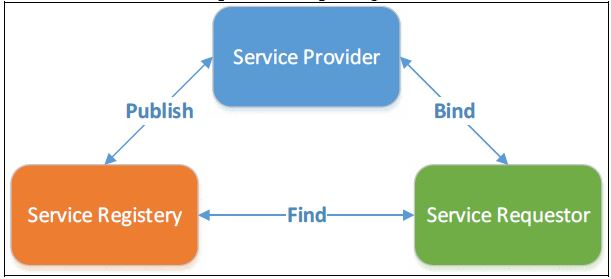
\includegraphics[width=1\textwidth]{figures/1arsitektur.JPG}}

\caption{Arsitektur web service.} 
\label{1arsitektur}
\end{figure}

Gambar \ref{1arsitektur} mendefinisikan arsitektur dari Web Services dimana pada Web Services sendiri terdiri dari Layanan Untuk 
Requestor, Registery dan juga Provider. Dimana kegiatan yang dilakukan untuk setiap layanan pada arsitektur tersebut ialah, `publish' 
untuk Service Registery dan Service Provider. `Bind' untuk Service Provider dan Serviice Requestor , dan juga `Find' untuk Service 
Registery dan Service Requestor. Pada Tabel \ref{1table} dipaparkan bahasa pemerograman yang sering digunakan dalam pembuatan frontend. 
Terdapat tiga komponen utama dari web service, komponen komponen tersebut antara lain :
service Provider, Service Requestor, Service Registry .


\begin{enumerate}
\item service Provider adalah penyedia web service yang berfungsi menyediakan kumpulan webService yang dapat diakses oleh USER atau pengguna.
\item Service Requestor Adalah aplikasi yang bertindak sebagai pengguan yang melakukan permintaan layanan berupa WebService kepada Service Provider.
\item Service Registry Adalah tempat dimana service provider mempublikasikan layanannya. pada arsitektur Webservice, service registry bersipat opsional\cite{kurniawan2015implementasi}.
\end{enumerate}


Pada Tabel \ref{1table} dipaparkan bahasa pemerograman yang sering digunakan dalam pembuatan frontend




\begin{table}[h]
\caption{Bahasa pemerograman yang sering digunakan di Frontend}
\centering
\begin{tabular}{ccccc}
\hline
one&two&three&four&five\\
\hline
Java&Phyton&PHP&Javascript&C++\\
\hline
\end{tabular}
\label{1table}
\end{table}





\chapter[Pengertian Web Service]
{pengertianwebservice}
%Resume tentang Pengertian Web Service

%Kelompok 2 D4 TI / 2B

%Alwan Suryansah				1164033 
%Dinda Ayu Pratiwi				1164034
%Kurnia Sandi					1164042
%Teduh Sanubari					1164054
%Wildan Khaustara Wijaksana		1164058

\documentclass[12pt]{article}
\usepackage{apacite}


\begin{document}

\title{Pengertian Web Service}
\maketitle

Web service ialah terobosan baru dalam sistem terdistribusi dengan Web yang menggunakan teknologi XML, dengan standar protokol  HTTP dan SOAP. Terobosan teknologi Web service muncul untuk mendukung sistem terdistribusi yang memiliki infrastruktur yang berbeda. Infrastruktur yang berbeda ini mampu dihubungkan dengan web service melalui XML sebagai teknologi yang mendukung integrasi berbagai paltform sistem dan aplikasi.
kbhbh
\section{Definisi}

\subsection{Hartati Deviana}
\paragraph{}
Web service adalah suatu komponen perangkat lunak self-containing dan aplikasi modular self-describing yang dapat disiarkan, dialokasikan, dan dijalankan di dalam web. Web service adalah teknologi yang mentransformasikan kemampuan internet dengan cara menambahkan beberapa kemampuan seperti kemampuan transactional web. Apa itu Transactional Web? Transactional Web yaitu kemampuan web dalam hal saling berinteraksi dengan pola program-to-program (P2P). Fokus web selama ini didominasi oleh komunikasi program-to-user dengan interaksi business-to-consumer (B2C), sedangkan transactional web akan didominasi oleh P2P dengan interaksi business-to-business (B2B). \cite{deviana2013penerapan}.

\subsection{Richards Robert}
\paragraph{}
Web service merupakan salah satu implementasi dari teknologi XML (Extensible Markup Language) pada proses pertukaran antara (data exchange) platform yang berbeda sercara berbeda.

\textit{"A Web service is a software system designed to support interoperable machine-to-machine interaction over a network. It has an interface described in a machine-processable format(specifically WSDL).Other systems interact with the Web service in a manner prescribed by its description using SOAP messages, typically conveyed using HTTP with an XML seriali zation in conjunction with other Web-related standards"}.

Menurut Richards, web service dapat digunakan untuk berkomunikasi antara mesin satu dengan mesin yang lain melalui interface perantara yang umumnya berupa WSDL(Web Service Definition Language), layanan ini biasa bekerja pada protokol HTTP dengan bentuk response dan request berupa SOAP messange. SOAP (Simple Object Access Protocol) adalah standar untuk bertukar pesan-pesan berbasis XML melalui jaringan komputer atau sebuah jalan untuk program yang berjalan pada suatu sistem operasi (OS) untuk berkomunikasi dengan program pada OS yang sama maupun berbeda dengan menggunakan HTTP dan XML sebagai mekanisme untuk pertukaran data. Format SOAP message adalah mengikuti frame XML yang terstandarisasi \cite{ihya2011pembuatan}. 

\subsection{Chen, Xi dan Zheng, Zibin dan Yu, Qi dan Lyu, Michael R}
\paragraph{}
Web Service adalah komponen perangkat lunak yang terintegrasi untuk mendukung interaksi antar mesin dengan mesin yang lainya ( komputer ) antar jaringan , layanan web service telah banyak digunakan untuk membangun suatu aplikasi yang berorientasi dengan layanan industri dan akademisi dalam beberapa tahun trakhir , jumlah layanan web yang tersedia untuk umum terus meningkat di internet , Namun  ini menyulitkan pengguna untuk memilih layanan yang tepat di antara banyaknya layanan web services\cite{chen2014web}.

\subsection{Witono, Timotius and Susanto, Raphael}
\paragraph{}
Pengertian sederhana web service adalah aplikasi yang dibuat agar dapat dipanggil atau diakses oleh aplikasi lain melalui internet atau intranet dengan menggunakan XML sebagai format pengiriman pesan. Web service digunakan saat pengguna akan mentransformasi sebuah logik atau sebuah class dan objek yang terpisah dalam satu ruang lingkup yang menjadi satu, sehingga tingkat keamanan dapat ditangani dengan baik\cite{witono201511}.

\subsection{Kurniawan, Erick}
\paragraph{}
Web Service adalah layanan yang tersedia di Internet. Web Service menggunakan format standar XML untuk pengiriman pesannya. Web Services juga tidak terikat kepada bahasa pemrograman atau sistem operasi tertentu (Ethan Cerami, 2002). Web Services adalah antar muka yang mendeskripsikan koleksi yang dapat diakses dalam jaringan menggunakan format standar XML untuk pertukaran pesan. Web Services mengerjakan tugas yang spesifik. Web Services dideskripsikan menggunakan format standar notasi XML yang disebut services description (Gottschalk, 2002)\cite{chen2014web}.

\subsection{Sarbini, Riska Nurtantyo}
\paragraph{}
Web service merupakan satuan diskrit dari fungsionalitas programatis yang diekspos 
kepada client via protokol komunikasi, dan format data standar bernama HTTP dan 
XML. Protokol ini mengatasi masalah komunikasi lintas internet dan lintas 
firewall tanpa beralih ke solusi superior yang memerlukan port-port komunikasi 
tambahan yang harus dibuka untuk akses eksternal. Dikarenakan web service mamiliki fungsi untuk menformat dan menguraikan pesan XML\cite{sarbini2015pengembangan}. 

\subsection{M. Shalahuddin dan Rosa A.S.}
\paragraph{}
Web Service merupakan suatu sistem yang menyediakan pelayanan yang dibutuhkan oleh klien. Klien dari web service tidak hanya berupa aplikasi web, tetapi juga bisa sebuah aplikasi enterprise. Jadi web service tidak sama dengan web server, bahkan sebuah aplikasi web pada web server dapat menjadi klien dari web service\cite{inayah2014aplikasi}.

\subsection{Gottschalk (2002)}
\paragraph{}
Web Service adalah teknologi yang mengubah kemampuan internet dengan menambahkan kemampuan transactional web, yaitu kemampuan web untuk saling komunikasi dengan pola program to program (P2P). Fokus web selama ini didominasi oleh komunikasi program to user dengan interaksi business to costumer (B2C), sedangkan stransactional web akan didominasi oleh P2P dengan interaksi business to business\cite{fauziah2014aplikasi}.


\subsection{Slameto, Andika Agus}
\paragraph{}
Web service adalah suatu sistem perangkat lunak yang dirancang untuk mendukung interoperabilitas dan interaksi antar sistem pada suatu jaringan. Web service digunakan sebagai suatu fasilitas yang disediakan oleh suatu web site untuk menyediakan layanan (dalam bentuk informasi) kepada sistem lain, sehingga sistem lain dapat berinteraksi dengan sistem tersebut melalui layanan-layanan (service)yang disediakan oleh suatu sistem yang menyediakan web service. Web service menyimpan data informasi dalam format XML, sehingga data ini dapat diakses oleh sistem lain walaupun berbeda platform, sistem operasi, maupun bahasa compiler\cite{slameto2015penerapan}.

\subsection{Jurnal Masyarakat Informatika}
\paragraph{}
web service adalah antarmuka yang mendeskripsikan sekumpulan operasi yang dapat diakses dalam sebuah jaringan melalui pesan XML yang telah distandartkan.xml iyalah bahasa markup yang sudah terintregrasi dengan web service. W3C mendefinisikan web service sebagai sebuah sistem perangkat lunak yang dirancang untuk mendukung inter operasi mesin ke mesin di sebuah jaringan.  Web service merupakan komponen perangkat lunak loosely coupled, dapat diguna ulang, membungkus fungsionalitas diskret, didistribusikan, dan diakses secara programatik melalui protokol internet standart . dan sangat di di perhatikan di bidang informatika \cite{saputra2integrasi}.

\subsection{Jurnal Sistem dan Teknologi Informasi}
\paragraph{}
Web service menurut World Wide Web Consortium (W3C) (2004), organisasi yang mengembangkan standar-standar dalam dunia web, mendefinisikan web service sebagai "\textit{“a software system designed to support interoperable machine-to-machine interaction over a network. It has an interface described in a machine-processable format (specifically WSDL). Other systems interact with the Web service in a manner prescribed by its description using SOAP messages, typically conveyed using HTTP with an XML serialization in conjunction with other Web-related standards.” }"(Lucky,2008).

Berdasarkan definisi dari W3C dapat disimpulkan bahwa web service merupakan aplikasi yang dibuat agar dapat dipanggil atau diakses oleh aplikasi lain melalui internet maupun intranet dengan menggunakan XML sebagai format pengiriman pesan\cite{prasetya2013perancangan}.

\subsection{Pengertian Web Service menurut Hartono, Fajar Fani and Hendry, H and Somya, Ramos}
\paragraph{}
Web Service dapat diartikan sebuah antar muka atau dalam bahas inggris yaitu interface  yang berarti menggambarkan sebuah sekumpulan operasi-operasi yang kemudian dapat diakses melalui jaringan, misalnya internet dalam bentuk pesan “Extensible Markup Language (XML)”. Web Service juga menyediakan standar komunikasi dalam berbagai software yang berbeda-beda, dan dapat berjalan di berbagai platform maupun framework\cite{hartono2013aplikasi}.

\subsection{Pengertian Web Service Menurut Kasaedja, Bramwell A and Sengkey, Rizal and Lantang, Oktavian A}
\paragraph{}
O’Reilly menerbitkan sebuah buku, David A Chappel dan Tyler Jewell sebagai penulis mengartikan bahwa web service adalah suatu kumpulan logika bisnis dalam internet yang dapat di akses melalui protocol internet. Dalam buku tersebut juga dijelaskan bahwa terdapat tiga komponen teknologi dalam Web service yaitu, Simple Object Acces Protocol (SOAP), Web Service Description Language (WSDL), dan Universal Description, Discoveri, Integration (UDDI)\cite{kasaedja2014rancang}.

\subsection{Hamdani, Hamdani and Haviluddin, Haviluddin and Darmawangsa, Ngurah Satria}
\paragraph{}
Web service diartikan sebagai sebuah antar muka (interface) yang menggambarkan sekumpulan operasi-operasi yang dapat diakses melalui jaringan, misalnya internet, dalam bentuk pesan XML. Web service diartikan sebagai sepotong atau sebagian informasi atau proses yang dapat diakses oleh siapa saja, kapan saja dengan menggunakan piranti apa saja, tidak terikat dengan sistem operasi atau bahasa pemrograman yang digunakan.

\subsection{Novi Nuari}
\paragraph{}
Webservice ialah suatu sistem perangkat lunak yang dibangun guna mendukung interaksi antar mesin dalam suatu jaringan. Webservice digunakan sebagai suatu fasilitas yang disediakan oleh suatu website untuk menyediakan layanan (dalam bentuk informasi) kepada mesin lain, sehingga mesin lain dapat berinteraksi dengan mesin tersebut melalui layanan-layanan (service) yang disediakan oleh provider\cite{nuari2014perancangan}.

\subsection{Wellem, Theophilus}
\paragraph{}
Web service merupakan suatu software sistem yang mendukung interaksi yang interoperable dari machine to machine melalui jaringan (World World Wide Consortium).  (Stencil Group). Dengan suksesnya Web service sebagai suatu standar teknologi software, memberikan peluang yang besar untuk pengembangan aplikasi terdistribusi melalui Internet.
Web service sebagai suatu standar teknologi software, memberikan peluang yang besar untuk pengembangan aplikasi terdistribusi melalui Internet. Saat ini Web service tidak hanya dapat diakses melalui komputer saja, tetapi juga dapat diakses melalui mobile device, seperti telepon seluler dan PDA, sehingga memungkinkan diciptakannya layanan mobile menggunakan Web service dan aplikasi mobile yang menggunakan Web service ini\cite{wellem2015perancangan}.

\subsection{Jurnal Informatika Kenali, Eko Win }
\paragraph{}
Menurut Gerami (2002) web services adalah suatu layanan-layanan yang disediakan oleh internet, dengan menggunakan pengiriman pesan format Extensible Markup Language (XML), dan tidak saling bergantung pada satu sistem operasi atau Bahasa pemrograman. Komponen dalam web service memiliki 3 arsitektur, dan masing-masing komponen tersebut adalah Service provider, Service requestor, dan Service registry\cite{kenali2015desain}. 

\subsection{Sigit, Haris Triono and Sulistiyono, Sulistiyono}
\paragraph{}
Web Service adalah bagian dari perangkat lunak yang membuat dirinya tersedia melalui internet dan menggunakan sistem pesan XML standar. XML digunakan untuk mengkodekan semua komunikasi ke Web Service. Misalnya, klien memanggil Web Service dengan mengirim pesan XML, kemudian menunggu tanggapan XML yang sesuai. Karena semua komunikasi ada dalam XML, Web Service tidak terkait dengan sistem operasi atau bahasa pemrograman manapun. Web Service adalah kumpulan protokol dan standar terbuka yang digunakan untuk pertukaran data antara aplikasi atau sistem\cite{sigit2017desain}.  

\section{Manfaat}

Layanan web memungkinkan penyedia layanan dan vendor untuk menjual layanan mereka dengan memublikasikannya
Yang di akses melalui World Wide Web.
Manfaat dari layanan web kita dapat berbagi data walaupun memiliki jarak yang jauh dan dapat mempermudah membagi suatu data dalam sebuah pekerjaan
interoperabilitas. Manfaat ini berasal dari antarmuka XML standar dan deskripsi akses
diberikan oleh WSDL (Web Services Description Language). Deskripsi WSDL sangat membantu dalam perusahaan
integrasi aplikasi, integrasi B2B (menyelesaikan tantangan antara bisnis dan bisnis partner, seperti customer, supplier, bank, dan jasa transportasi ) \cite{ferris2003web}.

\section{Arsitektur Web service}

\subsection{\textit{Service Oriented Architecure (SOA)} }

\paragraph{}
Konsep arsitektur yang mendasari teknologi Web service adalah Service Oriented Architecure (SOA), SOA mendefinisikan 3 peran berbeda yang menunjukkan peran dari masing-masing komponen dalam system, yaitu (W3C, 2004) :
\begin{itemize}
\item \textit{Service provider}, yaitu suatu entitas yang menyediakan interface terhadap sistem yang menjalankan suatu sekumpulan tugas tertentu.
\item \textit{Service requestor}, yaitu suatu entitas yang meminta/memperoleh (dan menemukan) \textit{software service} dalam rangka meyelesai kan suatu tugas tertentu atau menyediakan solusi bisnis tertentu.
\item \textit{Service registry}, yaitu entitas yang bertindak sebagai penyimpan (\textit{repository}) suatu \textit{software service} yang dipublikasikan oleh \textit{service provider}\cite{hidayat2014penerapan}.
\end{itemize}

\subsection{Jurnal Masyarakat Informatika}

\paragraph{}
Web service dibangun dari tiga komponen unsur utama, yaitu service provider, service registry, dan service requestor. Komponen-komponen tersebut saling berinteraksi melalui komponen web service itu sendiri, yang berupa deskripsi dan implementasi layanan dan prasarana. Dan juga terdapat tiga macam operasi yang memungkinkan komponen komponen tersebut untuk dapat saling berinteraksi, yaitu publish, find, dan bind. Keterkaitan antara peran, operasi, dan komponen web service \cite{saputra2integrasi}.

\subsection{Arsitektur RESTful Web services}
\paragraph{}
Berikut merupakan langkah-langkah yang dilakukan dalam model dasar RESTful Web services (HostBridge, 2009):
\begin{enumerate}
\item Query Request Provider melalui HTTP dengan menggunakan URI (Uniform Resource Identifier). Request menggunakan methods (metode) HTTP untuk menentukan apakah request tersebut dimaksudkan untuk Create (menciptakan), Read (membaca), Update (memperbarui), atau Delete (menghapus) data.
\item HostBridge mengembalikan sebuah dokumen dalam bentuk XML untuk Requester (pemohon) dengan CICS data enclosed\cite{arsana2014rancang}.
\end{enumerate}



\section{Kesimpulan}

\paragraph{}
Dari berbagai definisi tersebut dapat disimpulkan bahwa web service merupakan middleware sebuah internet yang memungkinkan berbagai sistem untuk saling berkomunikasi tanpa terpengaruh pada platform. Web service membungkus operasi-operasi ke dalam sebuah antarmuka yang ditulis dalam notasi XML. Antarmuka ini menyembunyikan detil implementasi dari layanan. Pertukaran informasi yang terjadi dalam web service juga menggunakan pesan dalam format XML \cite{saputra2integrasi}.


\bibliographystyle{apacite}
\bibliography{references}

\end{document}




% contoh aplikasi web service
% web service
% protokol
% port

% HTTP
% URL
% POST
% GET


\bibliographystyle{IEEEtran}.
\bibliography{references}.

\printindex

\end{document}
